\subsection{GUI (Mikkel)}
Et af kravene til programmet var, at det skulle være let at bruge. For at opnå dette, blev der valgt en grafisk brugergrænseflade, der let præsenterer informationer fra hele programmet.

\subsubsection{Startsiden}
Startsiden bliver styret af \texttt{StartController}. Herfra kan brugeren 'logge ind' på sin profil ved enten at indtaste sine initialer, eller vælge sig selv fra en liste. Det er herfra også muligt at lave en ny bruger, som får givet de indtastede initialer og fulde navn. Når man trykker på "Opret ny", vil man derefter blive logget ind som den nye bruger.

\begin{figure}[H]
    \centering
    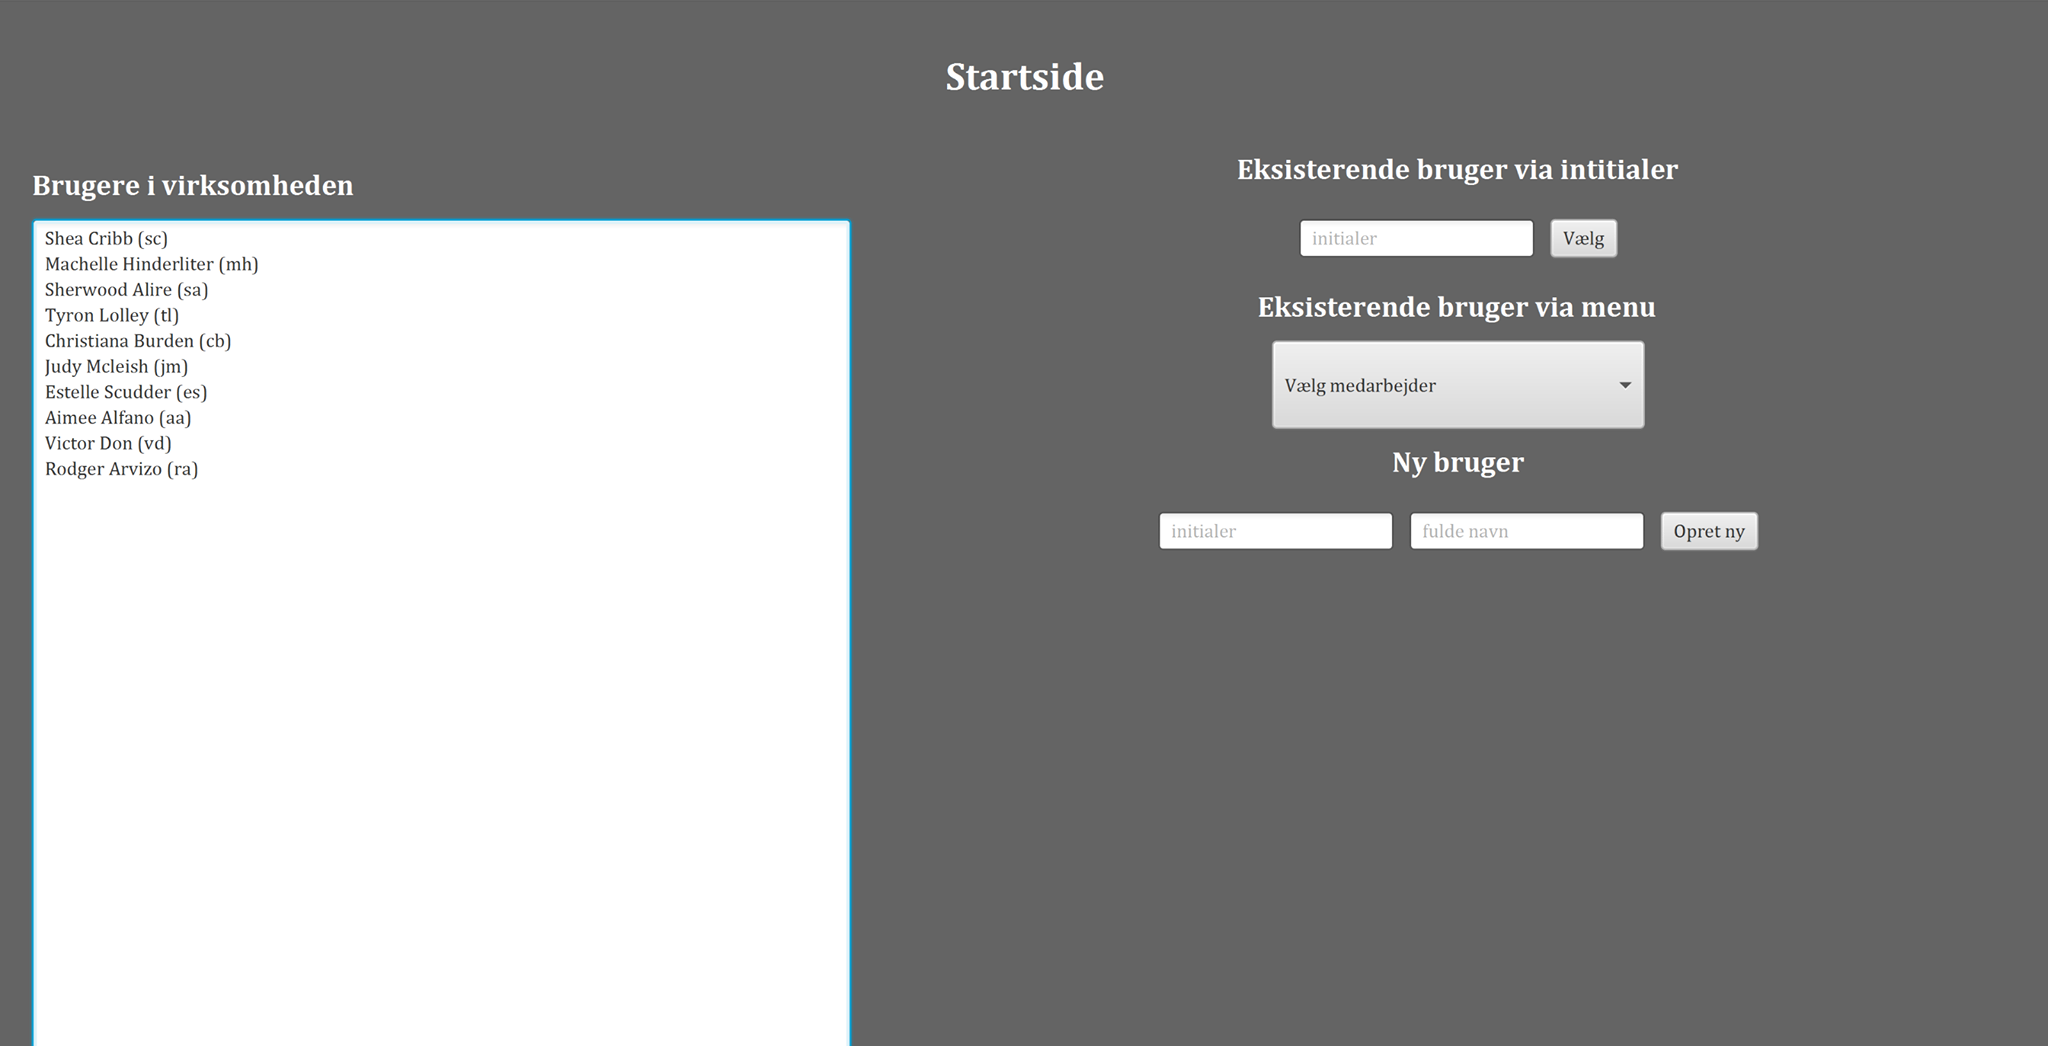
\includegraphics[width = \textwidth]{Figurer/startPage}
    \caption{Startsiden for programmet. Herfra kan man logge ind ved at vælge en bestemt bruger fra listen, eller indtaste deres initialer. Det er herfra også muligt at se alle brugere i virksomheden, eller lave en ny bruger ved at indtaste initialer og det fulde navn.}
    \label{fig:startPage}
\end{figure}

Åbner man startsiden, bliver metoden \texttt{goToStartPage} kørt, der opdaterer JavaFX objekterne på startsiden. Dette giver sig til udtryk bl.a. i listen over brugere i virksomheden, der bliver opdateret hver gang man kører \texttt{goToStartPage}. Dette skyldes, at \texttt{goToStartPage} laver en ny \texttt{sharedStartScene}, altså en ny scene til start siden. Når denne bliver skabt, køres metoden \texttt{initialize}, som opsætter logikken til knapperne på siden osv. I \texttt{initialize} bliver \texttt{refresh} kørt, der henter den nuværede liste over medarbejdere, og opdaterer bl.a. ComboBoxen der udgør drop-down menuen. \texttt{refresh} er her lidt overflødig, da man ikke kan ændre hvilke brugere der er i virksomheden uden at forlade startsiden. Den blev dog alligevel indført for at holde det samme format på alle siderne. 

Når man bliver logget ind, bliver feltet \texttt{activeEmployee} i klassen \texttt{App} sat til at være den valgte, eller nyskabte, bruger. Når man skifter til brugersiden, sker dette gennem metoden \texttt{goToUserPage}. 

\subsubsection{Brugersiden}
Når brugeren logger ind, kommer de ind på brugersiden, styret af \texttt{UserController}. Herfra kan brugeren se hvilke projekter og aktiviteter de er tilmeldt, samt hvilke tidsregistreringer de har udført. Det er også muligt at se tilgængeligheden for en bruger. Man kan herfra også gå hen til en anden bruger og se på deres info. I toppen af siden ses den aktive bruger, altså den bruger der er logget ind, udover to knapper der bringer dem tilbage til deres personlige brugerside, eller logger dem ud. Denne bar i toppen er konstant mellem alle sider man kan komme ind på, efter man er logget ind. Herfra kan brugeren gå videre til projekter, aktiviteter eller tidsregistreringer. Der er også mulighed for at lave nye af hver af disse. Dette fører en hen til deres respektive sider, hvor man kan indtaste flere informationer. I brugersiden er det ikke muligt at lave en normal aktivitet, men det er dog muligt at lave en statusaktivitet af den type som man vælger med drop-down menuen ved siden af. 

\begin{figure}[H]
    \centering
    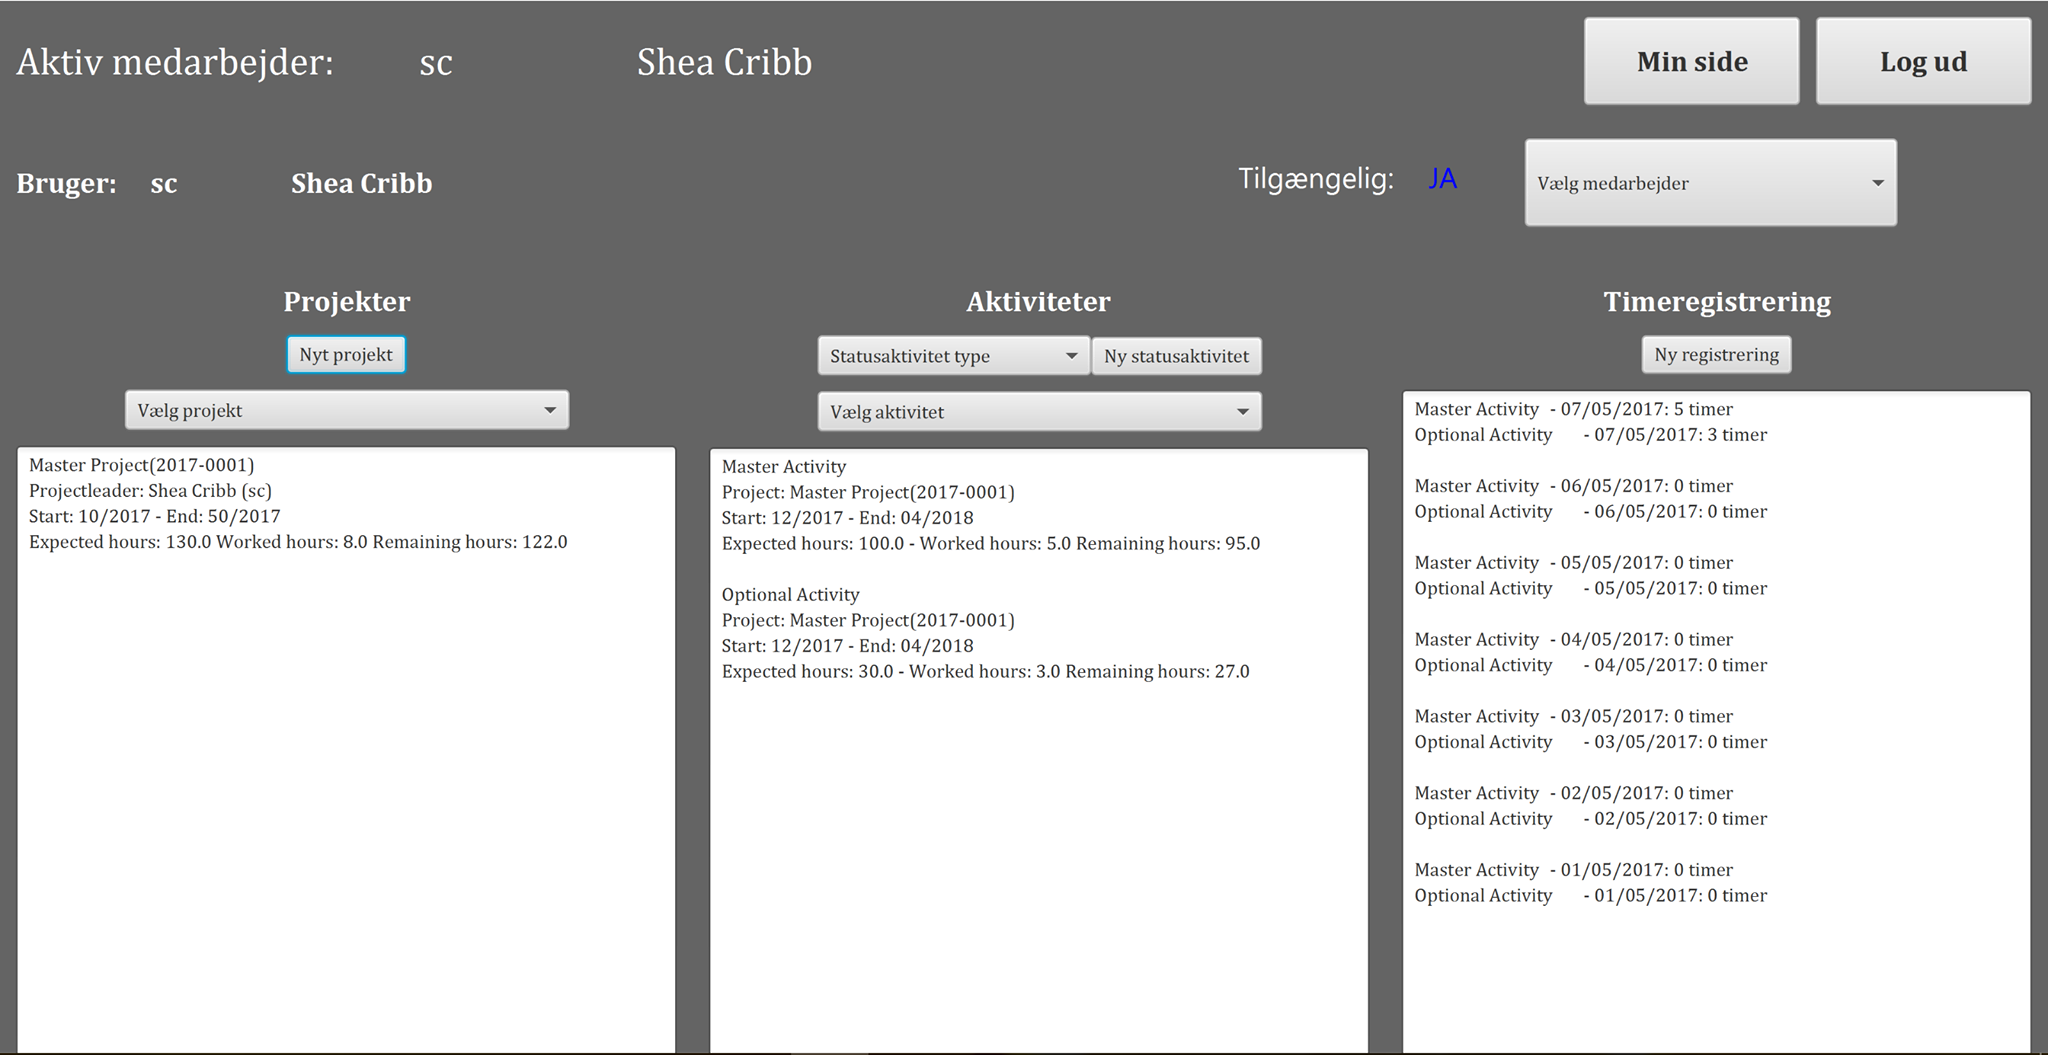
\includegraphics[width = \textwidth]{Figurer/userPage}
    \caption{Brugersiden for programmet. Herfra kan man se projekter og aktiviteter som brugeren er del af, samt deres tidsregistreringer. Det er herfra også muligt at lave nye projekter, status aktiviteter og tidsregistreringer. Man kan også vælge en anden bruger i virksomheden, og se deres brugerside.}
    \label{fig:userPage}
\end{figure}

Brugersiden bliver sat op gennem metoden \texttt{goToUserPage}, der fungerer ligesom den tidligere nævnte \texttt{goToStartPage}. Herfra bliver tekstfelter, drop-down menuer og knapper sat op. Baren i toppen af siden, der viser den bruger der er logget ind, viser informationerne for den bruger der er sat som \texttt{activeEmployee} i klassen \texttt{App}. Informationerne på brugersiden tilhører ikke nødvendigvis den aktive bruger, men tilhører brugeren markeret som \texttt{focusEmployee}. \texttt{focusEmployee} er et felt i klassen \texttt{Main}, der er en af klasserne der udgør den grafiske brugerflade. Dette blev valgt, da \texttt{focusEmployee} kun har noget at gøre med brugersiden, og intet med logikken af systemet. Går man til brugersiden gennem "Min side" knappen, eller gennem start siden, vil \texttt{focusEmployee} være den samme som \texttt{activeEmployee}. De bliver først forskellige når man, fra brugersiden, vælger en anden medarbejder fra drop-down menuen "Vælg medarbejder". Herfra bliver \texttt{focusEmployee} sat til at være den valgte medarbejder, men informationerne øverst i vinduet vil stadig tilhøre den bruger der er logget ind, da den fortsat viser \texttt{activeEmployee}. Listen over aktiviteter, projekter og tidsregistreringer vil vise disse tilhørende \texttt{focusEmployee}. Knapperne til at lave en ny statuaktivitet, nyt projekt eller en ny tidsregistrering er deaktiveret når man er inde på en brugerside hvor \texttt{focusEmployee} er forskellig fra \texttt{activeEmployee}. \texttt{focusEmployee} bliver dog kun brugt på brugersiden, og går man videre til enhver anden side vil man tilgå den som \texttt{activeEmployee}.

Metoden \texttt{refresh} i \texttt{userController} har her stor betydning, da det er den der opdaterer siden til at reflektere \texttt{focusEmployee}. \texttt{refresh} bliver her kørt, udover når siden initialiseres, også kørt hver gang der bliver valgt en medarbejder, som så bliver sat til \texttt{focusEmployee}. På den måde bliver kun de relevante felter opdateret, mens resten af siden kan forblive som den var før. 

% Måske noget om Tilgængelighed / hvordan data hentes ind, lidt voldsomt tho

\subsubsection{Projektsiden}
Der er flere måder at komme ind på projektsiden, styret af \texttt{ProjectController}. Enten kommer man ind ved at vælge et projekt fra brugersiden, ellers kommer man ind gennem aktivitetsiden. På projektsiden kan man se informationer for det valgte projekt, såsom start/slut dato, med videre. Der fremgår også en liste over aktiviteter tilhørende projektet, samt de medarbejdere der er tilskrevet aktiviteter i projektet. Man kan herfra også ændre på projektet hvis den aktive bruger er projektleder for det valgte projekt, samt generere projektrapporten og slette projektet. Derudover er det muligt at lave en ny aktivitet, som får navnet skrevet i tekst-boxen ved siden af. 

\begin{figure}[H]
    \centering
    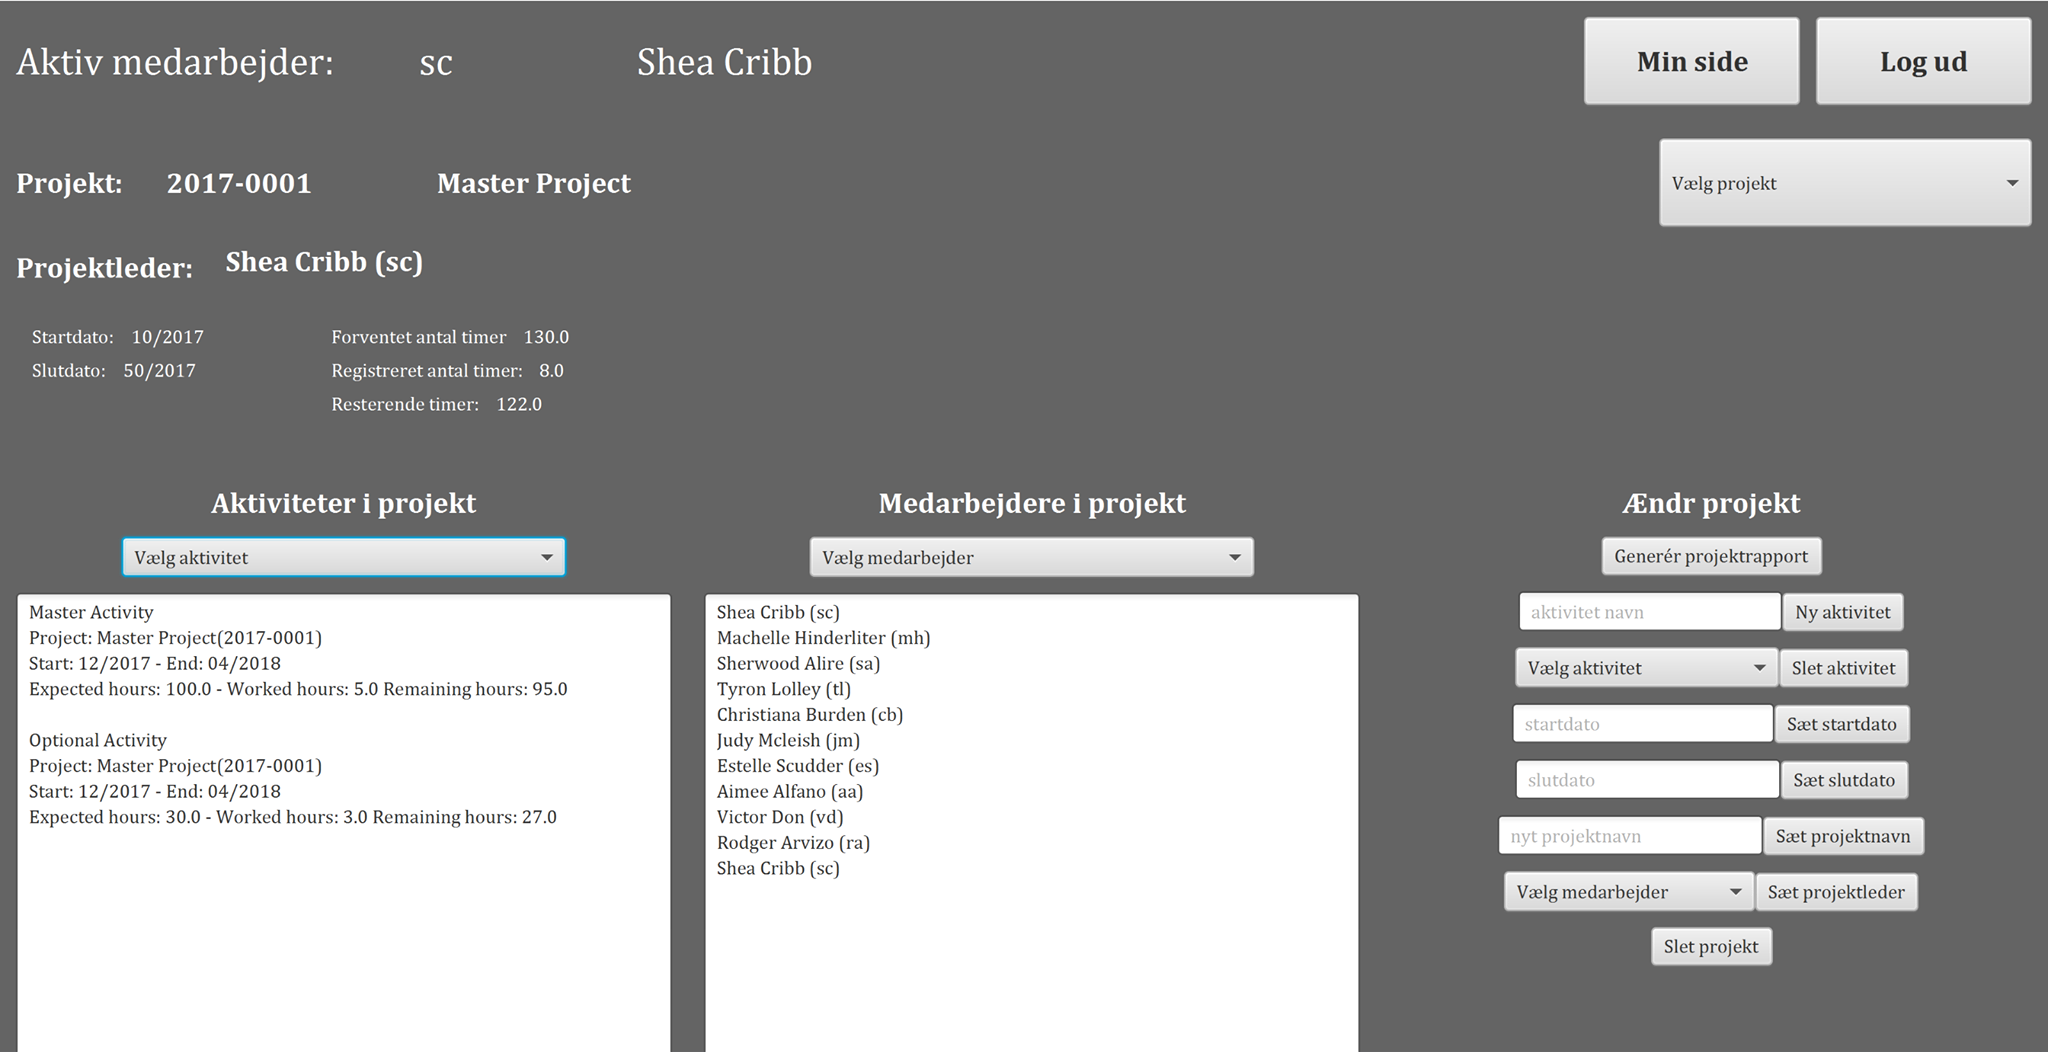
\includegraphics[width = \textwidth]{Figurer/projectPage}
    \caption{Projektsiden for programmet. Herfra kan man se de aktiviteter der indgår i projektet, samt medarbejdere der indgår i disse. Man kan derudover lave nye aktiviteter eller ændre i informationerne for projektet hvis man er tilskrevet som projektleder. Man kan også vælge et andet projekt, hvorefter man vil blive vist projektsiden for denne.}
    \label{fig:projectPage}
\end{figure}

Projektsiden bliver sat op gennem metoden \texttt{goToProjectPage}, der fungerer ligesom de tidligere nævnte funktioner der skifter side. \texttt{goToProjectPage} viser informationerne for den side der er blevet sat som \texttt{activeProject}, der bliver sat når man vælger et projekt. \texttt{activeProject} ligger i klassen \texttt{App}, men har en lidt anden funktionalitet for projektsiden end \texttt{activeEmployee} har for brugersiden. Når man skifter projekt inde fra projektsiden bliver \texttt{activeProject} sat ligesom \texttt{focusEmployee} i brugersiden, og metoden \texttt{refresh} køres, der opdaterer informationerne på siden til at tilhøre \texttt{activeProject}. For at få adgang til at ændre informationerne for projektet, skal \texttt{activeEmployee} være den samme bruger som projektets projektleder. Er \texttt{activeEmployee} ikke det, vil redigeringsknapperne og tekstefelterne blive inaktive. Går man videre til en aktivitetsside, tilgår man denne med hensyn til \texttt{activeProject}, da visse egenskaber på aktivitetssiden kun er tilgængelige for det tilhørende projekts projektleder. Bliver der lavet et nyt projekt, vil denne automatisk blive sat som tilhørende \texttt{activeProject}. Listen over medarbejdere findes ved at gå gennem alle medarbejdere i aktiviteter tilhørende projektet, og samler dem (samt projektlederen) i en liste.

% tjaaaaaaa...................

\subsubsection{Aktivitetsiden}
Aktivitetsiden kan tilgås direkte fra brugersiden, eller gennem projektsiden for projektet den tilhører, og bliver styret af \texttt{ActivityController}. Man kan her se informationerne for den valgte aktivitet, såsom forventet/registreret antal timer på aktiviteten, med videre. Man kan herfra også se den aktive brugers registrerede timer i aktiviteten, samt hvilke medarbejdere der er i aktiviteten. Det er herfra også muligt at søge assistance fra en anden medarbejder, hvorefter denne vil blive tilføjet til aktiviteten (hvis ikke de allerede er det). Der er en drop-down menu, hvorfra man kan vælge at gå til en af de andre aktiviteter der tilhører det samme projekt, udover en knap der tager brugeren tilbage til projektsiden for det projekt som aktiviteten tilhører. Hvis den aktive bruger er projektleder på det projekt som aktiviteten tilhører, er det muligt at ændre i aktivitetens informationer, samt generere en rapport eller slette aktiviteten. 

\begin{figure}[H]
    \centering
    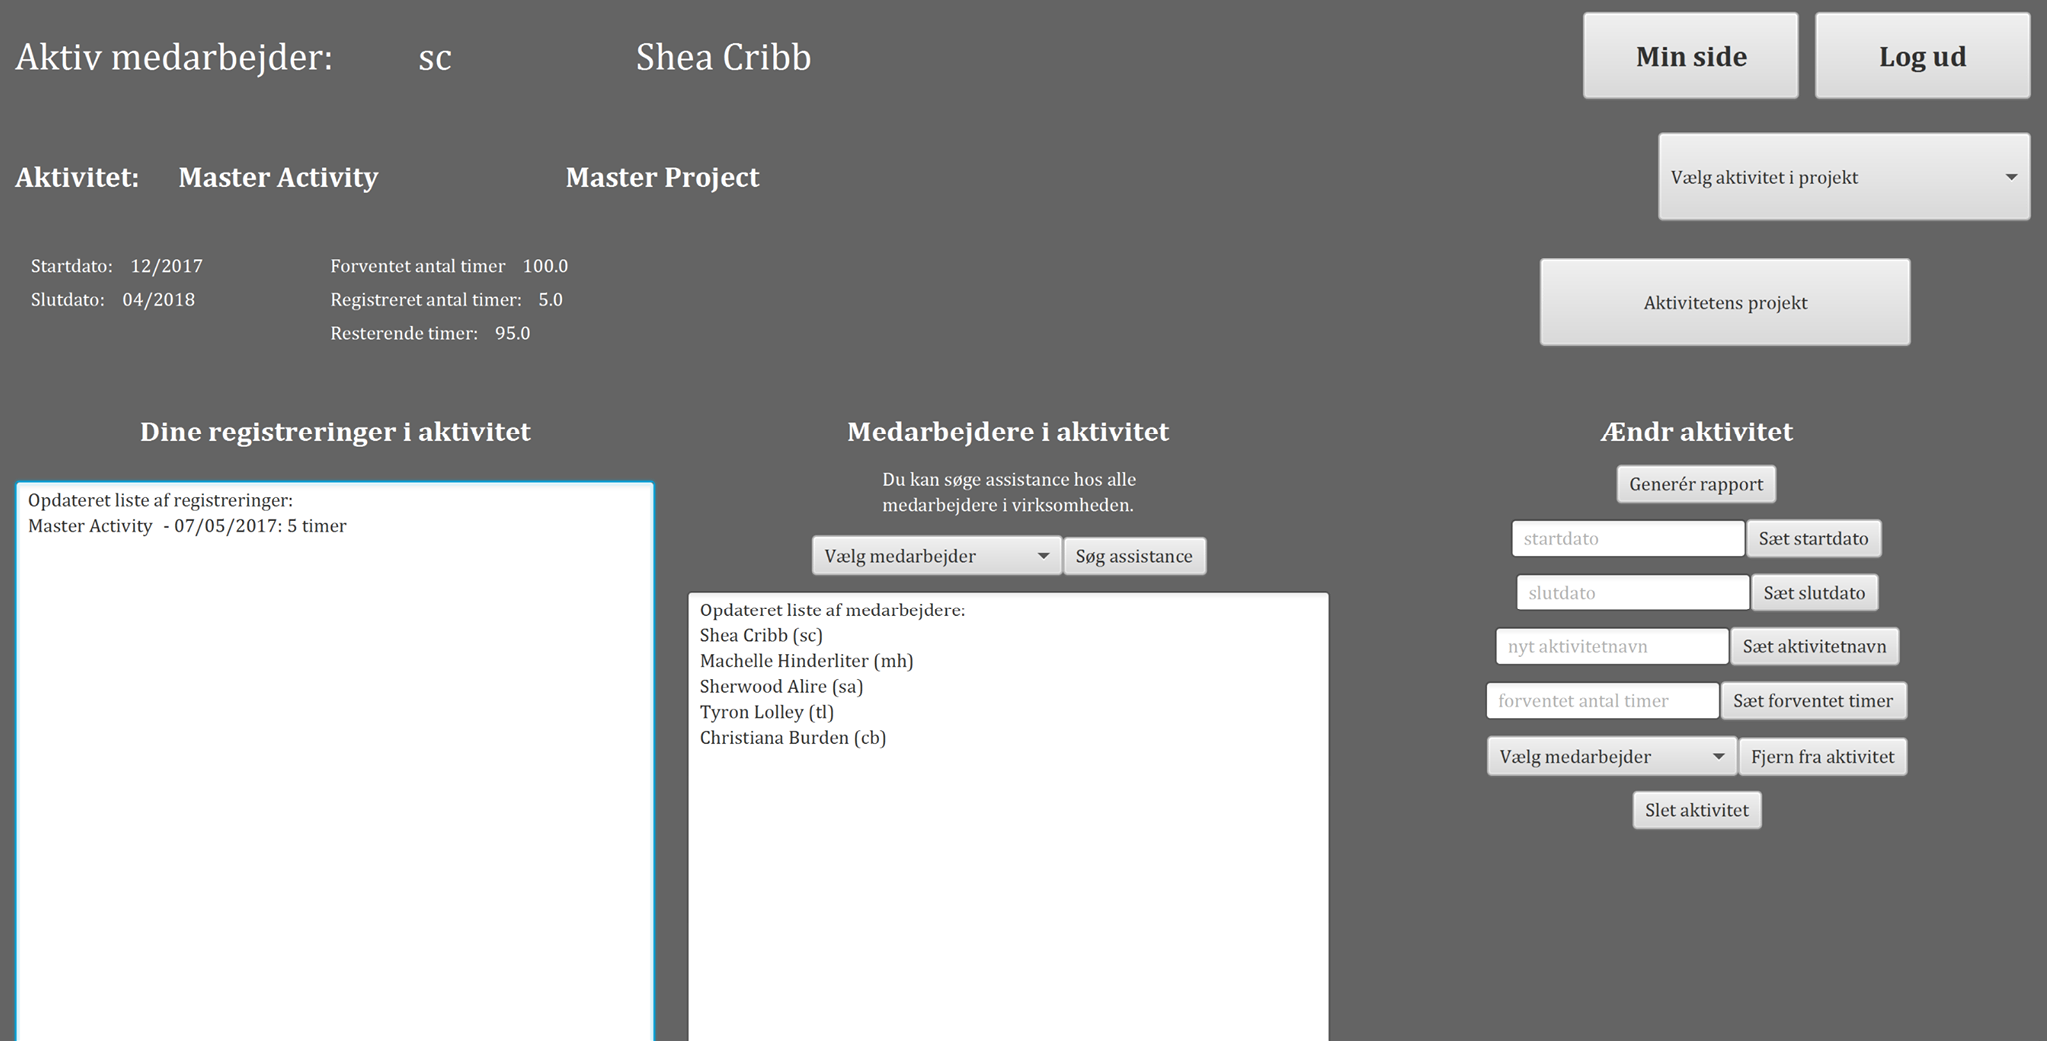
\includegraphics[width = \textwidth]{Figurer/activityPage}
    \caption{Et eksempel på en aktivitetside. Man kan herfra se informationerne for aktiviteten, samt de seneste tidsregistreringer, den aktive bruger har lavet på projektet. Man kan også vælge en anden aktivitet fra projektet, og gå til dens side.}
    \label{fig:activityPage}
\end{figure}

Ligesom de andre sider, bliver aktivitetsiden sat op gennem \texttt{goToActivityPage}, og informationerne på siden opdateret gennem \texttt{refresh}. Den aktivitet der bliver vist bliver sat når man vælger en aktivitet på en af de andre sider, og betegnes \texttt{activeActivity} i klassen \texttt{App}. Knappen "Aktivitetens projekt" tager en tilbage til projektet markeret som \texttt{activeProject}, der bliver sat til at være det projekt der tilhører \texttt{activeActivity}. Vælger man en anden aktivitet fra aktivitetsiden, bliver denne sat som \texttt{activeActivity}, og \texttt{refresh} bliver kørt. Hvis \texttt{activeEmployee} ikke er projektleder på aktivitetens projekt, vil knapper og tekstfelter relaterede til at ændre aktivitetens informationer blive inaktive

Hvis aktiviteten er en statusaktivitet, har den ikke noget projekt den er en del af. Da dette er tilfældet, er der ikke nogen projektleder for aktiviteten. Det er i stedet for muligt for alle at ændre på statusaktivitetens informationer. Der er dog visse felter der er inaktive, såsom ændring af statusaktivitetns navn.

%%%%%%%%%%%%%% MAYBE MORE??????????

\subsubsection{Tidsregistrering}
Tidsregistreringsiden kan kun tilgås gennem brugerens egen brugerside, dvs. hver bruger kan kun se sine egne registreringer. Fra registreringssiden kan man registrere timer arbejdet på en valgt aktivitet, og til en indtastet dato. Man kan derudover se tidligere registreringer i uge-intervaller. 

\begin{figure}[H]
    \centering
    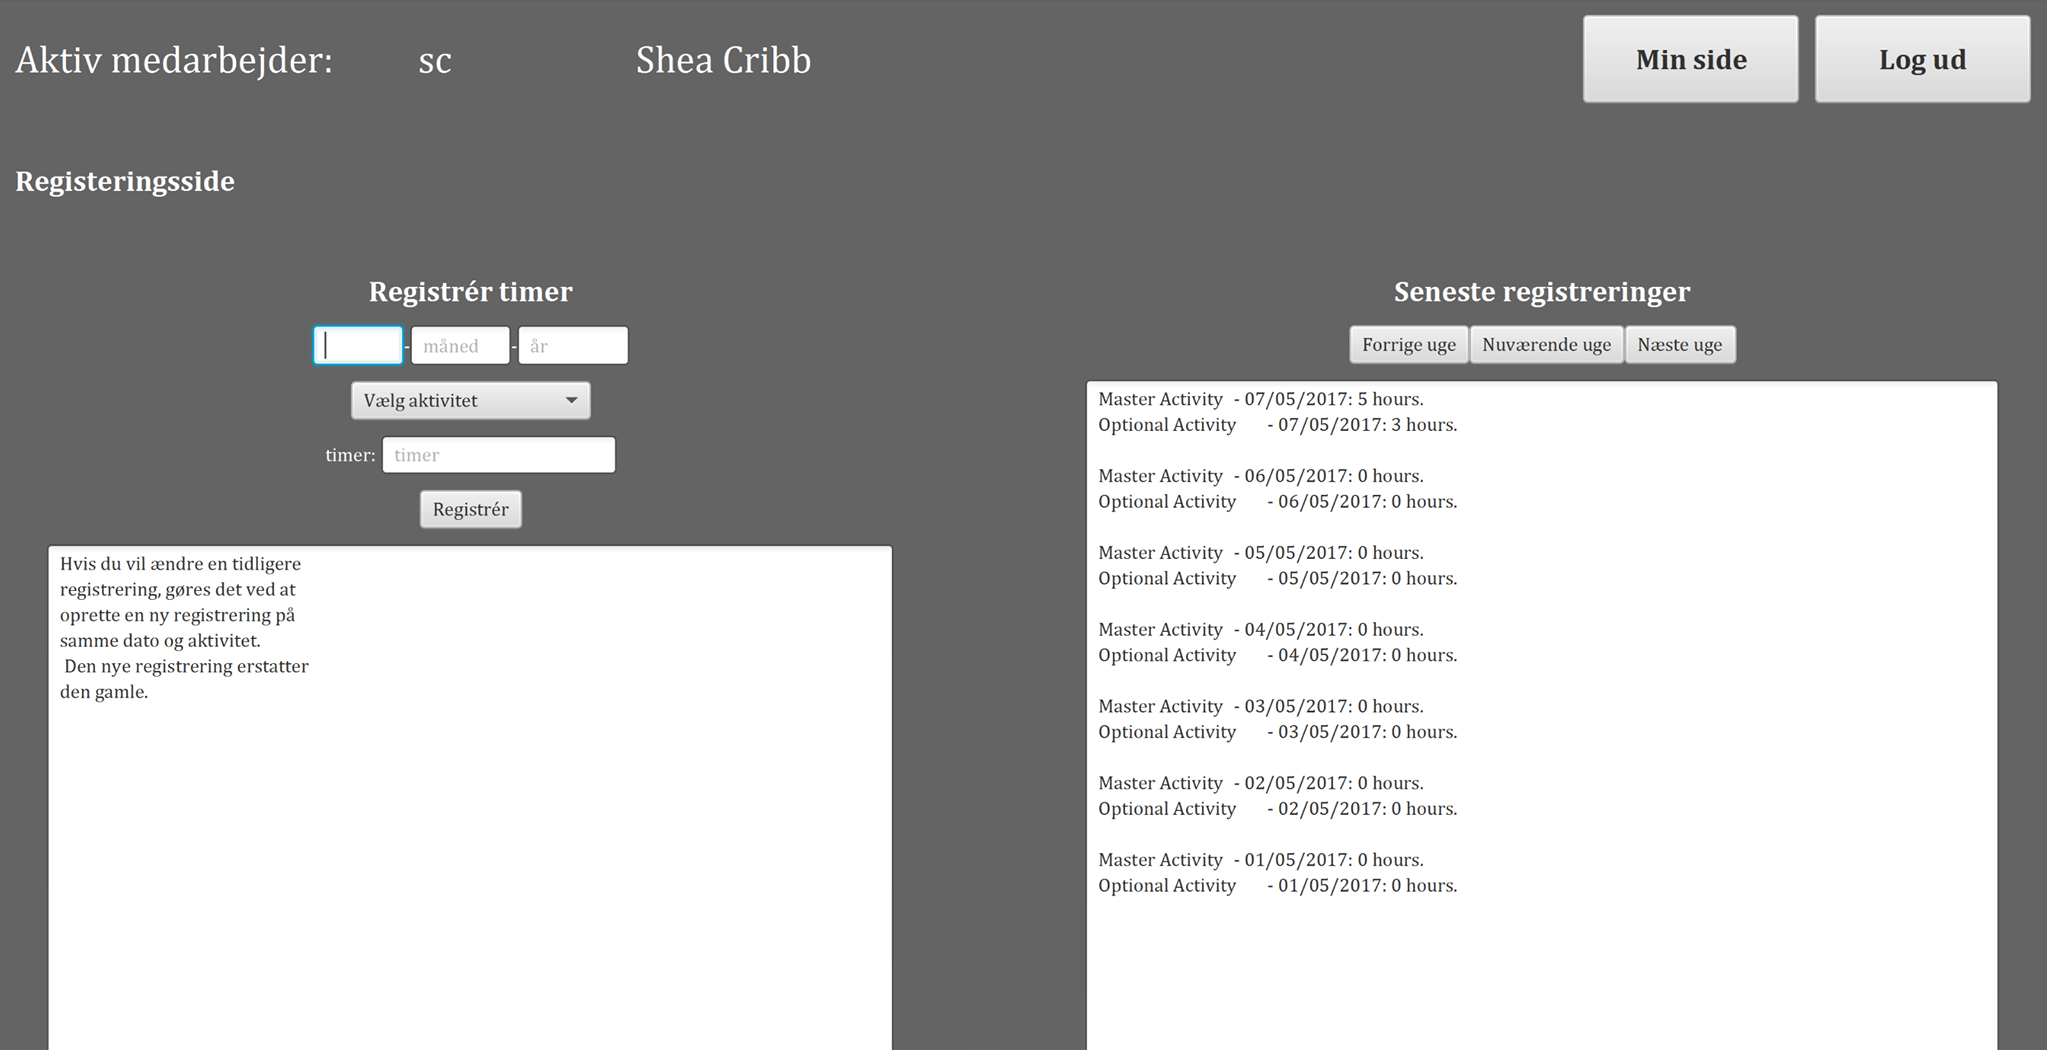
\includegraphics[width = \textwidth]{Figurer/registrationPage}
    \caption{Tidsregistreringssiden for programmet. Herfra kan man indtaste hvor mange timer man har arbejdet, hvilken dag man har arbejdet, samt hvilken aktivitet man har arbejdet på.}
    \label{fig:registrationPage}
\end{figure}

Tidsregistreringssiden bliver sat op gennem \texttt{goToRegistrationPage}. Herfra bliver siden sat op, og informationerne bliver udfyldt af metoden \texttt{refresh}. Tidsregistreringerne bliver sat ved at hente brugerens aktiviteter. 